%% ============================================================================
%% EchoPulse AI -- version para CEUR-WS (clase ceurart)
%% Fusión: ECHOPULSE_CLEANED (documento base, .docx) + versión IEEE (LaTeX)
%% Requisitos NALEF 2026: 5-8 páginas, inglés, plantilla CEURART,
%% sin números de página ni encabezados (no usar las opciones twocolumn ni hf).
%% ============================================================================
\documentclass[]{ceurart}

%% One can fix some overfulls
\sloppy
\usepackage{amsmath,amssymb,amsfonts}
\usepackage{graphicx}
\usepackage{textcomp}
\usepackage{xcolor}
\usepackage{url}
\usepackage{booktabs}
\usepackage{microtype}
\emergencystretch=1em

%% Buscar imágenes tanto en figures/ como en la raíz del proyecto de Overleaf.
\graphicspath{{figures/}{./}}

%% ---- notación matemática ----
\newcommand{\vect}[1]{\boldsymbol{#1}}
\newcommand{\mat}[1]{\mathbf{#1}}
\newcommand{\Real}{\mathbb{R}}
\newcommand{\softmax}{\operatorname{softmax}}
\newcommand{\LayerNorm}{\operatorname{LayerNorm}}
\newcommand{\GELU}{\operatorname{GELU}}
\newcommand{\cosine}{\operatorname{cos}}

\begin{document}

%% ---- nota de copyright exigida por la convocatoria (pie de la pág. 1) ----
\copyrightyear{2026}
\copyrightclause{Copyright for this paper by its authors.
  Use permitted under Creative Commons License Attribution 4.0
  International (CC BY 4.0). NALEF 2026, Cartagena, Colombia.}

%% ---- evento (CEUR-WS lo imprime en la primera página) ----
%% EDITOR: confirmar el nombre oficial del workshop/volumen CEUR-WS.
\conference{NALEF 2026: 9th Encuentro de Semilleros de Investigación,
  October 2026, Cartagena, Colombia}

%% ---- título ----
\title{EchoPulse AI: A Hybrid Local Data Architecture for Multimodal Music
  Recommendation}
\subtitle{Integrating WASABI, MSD, and TalkPlay Datasets}

%% ---- autores ----
\author[1]{John Kennedy Landazuri Sandoval}[%
orcid=0009-0004-7437-2779,
email=john.landazuri@estudiante.fup.edu.co,
]
\cormark[1]
\fnmark[1]

\author[1]{Cristian Camilo Ordoñez Quintero}[%
orcid=0000-0003-4157-1611,
email=camilo.ordonez@docente.fup.edu.co,
]
\cormark[2]
\fnmark[1]

\author[2]{Hugo Armando Ordoñez Erazo}[%
orcid=0000-0002-3465-5617,
email=hugoordonez@unicauca.edu.co,
]
\fnmark[1]

\author[1]{Cristian Méndez Rodríguez}[%
orcid=0000-0002-4489-2712,
email=cristian.mendez@docente.fup.edu.co,
]

\address[1]{IMS Research Group, Fundación Universitaria de Popayán,
  Popayán, Cauca, Colombia}
\address[2]{Research Group on Technology and Information Management (GT),
  Universidad del Cauca, Popayán, Cauca, Colombia}

\cortext[1]{Corresponding author.}
\cortext[2]{Corresponding author.}
\fntext[1]{These authors contributed equally.}

%% ---- resumen ----
\begin{abstract}
Most music recommendation systems share a rather stubborn flaw: they keep
feeding the popular while starving emerging artists, because traditional
algorithms obsess over popularity signals and largely ignore actual content
affinity. This paper introduces EchoPulse AI, a locally deployed multimodal
recommender that tackles this visibility gap head-on. The system processes
lyrical, acoustic, metadata and conversational data through a Triple-Encoder
Transformer architecture, and consolidates heterogeneous datasets (WASABI,
Million Song Dataset, Lyrics 1950--2019 and TalkPlayData-2) through a
five-stage local pipeline. We chose local deployment over cloud infrastructure
because of cost constraints and unstable connectivity in the region; instead
of treating these limits as a weakness, they forced a design that prioritises
efficiency, reproducibility and zero cloud dependency. The core methodology
relies on a deliberately curated Master Table of 5,710 tracks with complete
multimodal coverage, designed as a controlled proof of concept that isolates
the cold-start problem. Experimental evaluation against collaborative
filtering, BERT4Rec and SASRec baselines shows competitive accuracy
(Hit@10\,=\,0.312) while improving Intra-List Diversity by 45.3\% and, most
importantly, Emerging Artist Discovery by 157.9\%. Core retrieval components
run at sub-250\,ms latency on consumer hardware. The current setup has clear
limitations: it mostly recommends English-language content, needs adaptation
for Spanish-language music, and requires further work to become adaptable to
arbitrary music databases. Scaling to industrial catalogues and running online
user studies are the key next steps.
\end{abstract}

%% ---- palabras clave ----
\begin{keywords}
Multimodal recommendation \sep
Transformer architecture \sep
Local data lakehouse \sep
Music information retrieval \sep
Cold-start problem \sep
Conversational AI \sep
Generative evaluation \sep
Popularity bias mitigation
\end{keywords}

\maketitle

%% ============================================================================
\section{Introduction}
\label{sec:introduction}

Digital streaming totally reshaped the music business. Global revenues hit USD
29.6 billion in 2024, showing massive growth in the streaming
era~\cite{ifpi2024report}. Yet this economic expansion has not exactly trickled
down to emerging artists, who still face a brutal visibility gap in an
increasingly concentrated digital landscape. For independent musicians, the
boom often feels like an illusion. The first author spent 14 years playing
drums in various bands across Colombia, and the reality on the ground is
pretty stark: new artists just do not get recommended. Not because their music
lacks quality, but because algorithms systematically favour established acts.

Most platforms still lean heavily on collaborative filtering. They track who
clicks what and amplify the hits. That works fine for global superstars, but
it falls apart when faced with the cold-start problem~\cite{schein2002methods,
adomavicius2005toward}. If a new track has no play history, the algorithm
ignores it, which creates a vicious feedback loop funneling all attention
toward the same handful of songs. In Latin American music scenes the situation
is even worse: local artists are not just competing with global hits, they are
drowning in a sea of algorithmically generated background music.

Content-based approaches offer a way out. By looking at actual lyrics, acoustic
properties and metadata of a song, it becomes possible to recommend based on
what the music actually sounds like~\cite{ricci2015recommender}. Comprehensive
treatments of recommender systems theory~\cite{aggarwal2016recommender} provide
the foundation on which modern Transformer-based approaches are built. The
seminal work ``Attention Is All You Need'' by Vaswani
et~al.~\cite{vaswani2017attention} particularly inspired this project. Its
ability to map long-range dependencies makes Transformers ideal for capturing
the complex structure of musical content~\cite{baltruvsaitis2019multimodal}.

This paper introduces EchoPulse AI. We built it as a locally deployed
multimodal recommender within the IMS Research Group at Fundación Universitaria
de Popayán. Why local? Simple answer. The research group had a limited budget
for cloud services, and internet connectivity in the region is notoriously
unstable. Instead of seeing these constraints as a weakness, the team used them
to force a design that prioritises efficiency, reproducibility and zero cloud
dependency.

Three main contributions emerge from this work. First, a hybrid local data
architecture is proposed and demonstrated: a five-stage paradigm that merges
messy, heterogeneous music datasets without needing AWS or GCP. Second, a
Triple-Encoder Transformer is designed and empirically validated; it processes
lyrics, audio and conversational data through specialised modules, backed by
strict mathematical formulations. Third, an end-to-end evaluation is provided,
demonstrating that one can drastically improve diversity and surface emerging
artists without tanking accuracy metrics.

Building the Master Table was easily the hardest part of this project. The team
had to reconcile completely different identifier systems, handle massive
amounts of missing data, and force four distinct datasets into a single, clean
collection of 5,710 tracks. That data-engineering struggle directly shaped the
architecture described in the following sections.

The rest of the paper walks through the approach step by step.
Section~\ref{sec:framework} covers the theoretical framework and related work.
Section~\ref{sec:methodology} dives into the five-stage pipeline and the model
architecture. Hardware setup and metrics are detailed in
Section~\ref{sec:results}, followed by an analysis of architectural
generalisation and limitations in Section~\ref{sec:discussion}. Finally,
Section~\ref{sec:conclusion} wraps up the findings.

%% ============================================================================
\section{Framework}
\label{sec:framework}

\subsection{Theoretical Framework}
\label{sec:theoretical}

\subsubsection{Attention and Transformer Architecture}
Back in 2017, Vaswani and colleagues dropped a paper that changed everything.
Their Transformer architecture~\cite{vaswani2017attention} introduced a
self-attention mechanism computed as
\begin{equation}
\text{Attention}(\mat{Q},\mat{K},\mat{V})
  = \softmax\left(\frac{\mat{Q}\mat{K}^\top}{\sqrt{d_k}}\right)\mat{V}
\label{eq:attention}
\end{equation}
The math looks intimidating at first glance, but the idea is straightforward:
one has query, key and value matrices ($\mat{Q}$, $\mat{K}$, $\mat{V}$), and
the model figures out which parts of the sequence matter most. This works
surprisingly well for music because songs have structure---verses, choruses,
bridges---that Transformers can pick up on.

\subsubsection{Multimodal Fusion Principles}
One cannot look at a single aspect of a song: lyrics matter, acoustic features
matter, metadata matters. Baltru{\v{s}}aitis
et~al.~\cite{baltruvsaitis2019multimodal} laid out the theoretical groundwork for
combining
multiple data sources. Cross-modal attention mechanisms appeared in
vision-language work such as ViLBERT~\cite{lu2019vilbert} and
LXMERT~\cite{tan2019lxmert}, and we adapted those theoretical concepts for
cross-attention fusion in music. Early fusion often struggles with aligning
heterogeneous feature spaces, while late fusion fails to capture deep
inter-modal correlations.

\subsubsection{Local Data Architecture Theory}
The Lakehouse paradigm is the current reference point in data management.
Armbrust et~al.~\cite{armbrust2020delta} showed how to get data-lake
flexibility together with data-warehouse transactional capabilities, through
Delta Lake, Apache Iceberg and Apache Hudi, which handle ACID transactions over
object storage. Our implementation adapts these principles locally, using
parquet-based storage with manual versioning, schema validation and snapshot
isolation; data-versioning approaches discussed by Pimentel
et~al.~\cite{pimentel2021dataversioning} informed that design. The result is
reproducibility and traceability without needing AWS or GCP.

\subsection{Background and Related Work}
\label{sec:background}

\subsubsection{Sequential Recommendation Models}
BERT4Rec~\cite{sun2019bert4rec} took Transformers further with bidirectional
encoding, improving accuracy but also inheriting all the popularity bias of the
training data. SASRec~\cite{kang2018self} went a different route with
self-attention for sequential recommendation. Both became our baseline
comparisons.

\subsubsection{Multimodal Music Recommendation}
Tzanetakis and Cook~\cite{tzanetakis2002genre} did early work on genre
classification that everyone still builds on, and
M{\"u}ller~\cite{mueller2015fundamentals} formalised the
music-information-retrieval pipeline
we follow for feature extraction. For fusing audio with text, Porcaro
et~al.~\cite{porcaro2021diversity} explored techniques for evaluating diversity
in music recommenders. On the emotional side, Russell's circumplex
model~\cite{russell1980circumplex} and Eerola and Vuoskoski's
review~\cite{eerola2013review} help map acoustic and lyrical features to
emotional dimensions.

\subsubsection{Mitigating Popularity Bias}
Previous approaches to mitigating popularity bias primarily rely on
post-processing re-ranking, inverse propensity weighting, or adversarial
debiasing during the collaborative-filtering
stage~\cite{kaminskas2016diversity}. While these methods adjust the final
output distribution, they do not solve the root cause: the fundamental lack of
content representation for cold-start items. Conversely, multimodal recommender
systems have explored early and late fusion~\cite{baltruvsaitis2019multimodal}.
Our demonstration provides empirical evidence that cross-attention explicitly
maps lyrical semantics onto acoustic properties, producing a robust latent
representation that inherently bypasses historical popularity signals and
directly addresses the limitations of prior unimodal and late-fusion
approaches.

\subsubsection{Conversational Recommendation Systems}
TalkPlay~\cite{choi2025talkplaydata2} uses large language models for music
recommendation through natural language. It is compelling, but lacks structured
multimodal integration and does not rigorously evaluate its generative
components. We extended this line of work by building a dedicated
conversational encoder trained on TalkPlayData-2 and by proposing evaluation
metrics for intention-aware
recommendation~\cite{gao2021advances,christakopoulou2016conversational}.
Retrieval-augmented
generation frameworks~\cite{lewis2020rag,gao2023rag} provided the
methodological foundation for integrating external knowledge with generative
models, which is exactly what we needed for connecting user intent to specific
songs.

\subsubsection{Foundational Datasets}
The datasets we used are pretty much the foundation for this kind of research:
\begin{itemize}
  \item \textbf{WASABI Dataset}~\cite{tikat2021wasabi}: lyrical content and
    cultural metadata for over 2 million commercially released songs, covering
    1922 to 2022.
  \item \textbf{Million Song Dataset (MSD)}~\cite{bertin2011million}: 26
    continuous acoustic features---tempo ($\tau$), energy ($E$), valence ($V$),
    danceability ($D$), loudness ($L$)---for 280,000 tracks, normalised to
    $[0,1]$~\cite{spotify2023audio}.
  \item \textbf{Lyrics 1950--2019}~\cite{moura2020lyrics}: thematic and
    emotional metadata from lyrical analysis across six decades, encoded as
    sentiment vectors $\vect{s}\in\Real^{6}$ based on the circumplex affect
    model~\cite{russell1980circumplex}.
  \item \textbf{TalkPlayData-2}~\cite{choi2025talkplaydata2}: a conversational
    corpus with around 16,000 structured dialogues mapping user intentions to
    song selections.
\end{itemize}

\subsection{Theoretical Model Construction and Hypotheses}
\label{sec:hypotheses}

Based on the theoretical framework, we construct a hybrid model that shifts the
recommendation paradigm from purely interaction-based collaborative filtering
to a content-aware multimodal approach. We posit the following hypotheses.

\textbf{Hypothesis 1 (H1 --- Multimodal Fusion Superiority).} Fusing lyrical,
acoustic and conversational modalities via cross-attention mechanisms provides
measurable benefits in capturing user intent compared to early/late fusion or
unimodal baselines.

\textbf{Hypothesis 2 (H2 --- Mitigation of Popularity Bias).} A content-based
multimodal approach inherently avoids popularity bias, significantly improving
Intra-List Diversity (ILD) and Emerging Artist Discovery (EAD).

To formalise H1 and H2, the theoretical model integrates a Hybrid Scoring
Function:
\begin{equation}
S(q,c) = \alpha \cdot \cosine(\vect{e}_q, \vect{e}_c)
       + \beta \cdot \left(1 - \frac{\|\vect{f}_q - \vect{f}_c\|_2}
       {\|\vect{f}_q\|_2 + \|\vect{f}_c\|_2}\right)
       + \gamma \cdot \frac{|T_q \cap T_c|}{|T_q \cup T_c|}
\label{eq:scoring}
\end{equation}
where $\alpha=0.4$ prioritises semantic embeddings, $\beta=0.3$ emphasises
acoustic continuity, and $\gamma=0.3$ enforces lexical filtering through
Jaccard similarity over the token sets $T_q$ and $T_c$.

%% ============================================================================
\section{Methodology}
\label{sec:methodology}

\subsection{Data Architecture Overview: Five-Stage Local Pipeline}
EchoPulse AI follows a five-stage data pipeline, adapting established MLOps
principles for local deployment. Figure~\ref{fig:architecture} maps the entire
journey from raw, heterogeneous data sources to local deployment, complete with
an evaluation feedback loop. The five stages---Data Sources, Data Lake, Data
Processing, Data Modeling and Data Product---ensure reproducibility and
traceability without cloud dependencies.

\begin{figure}
\centering
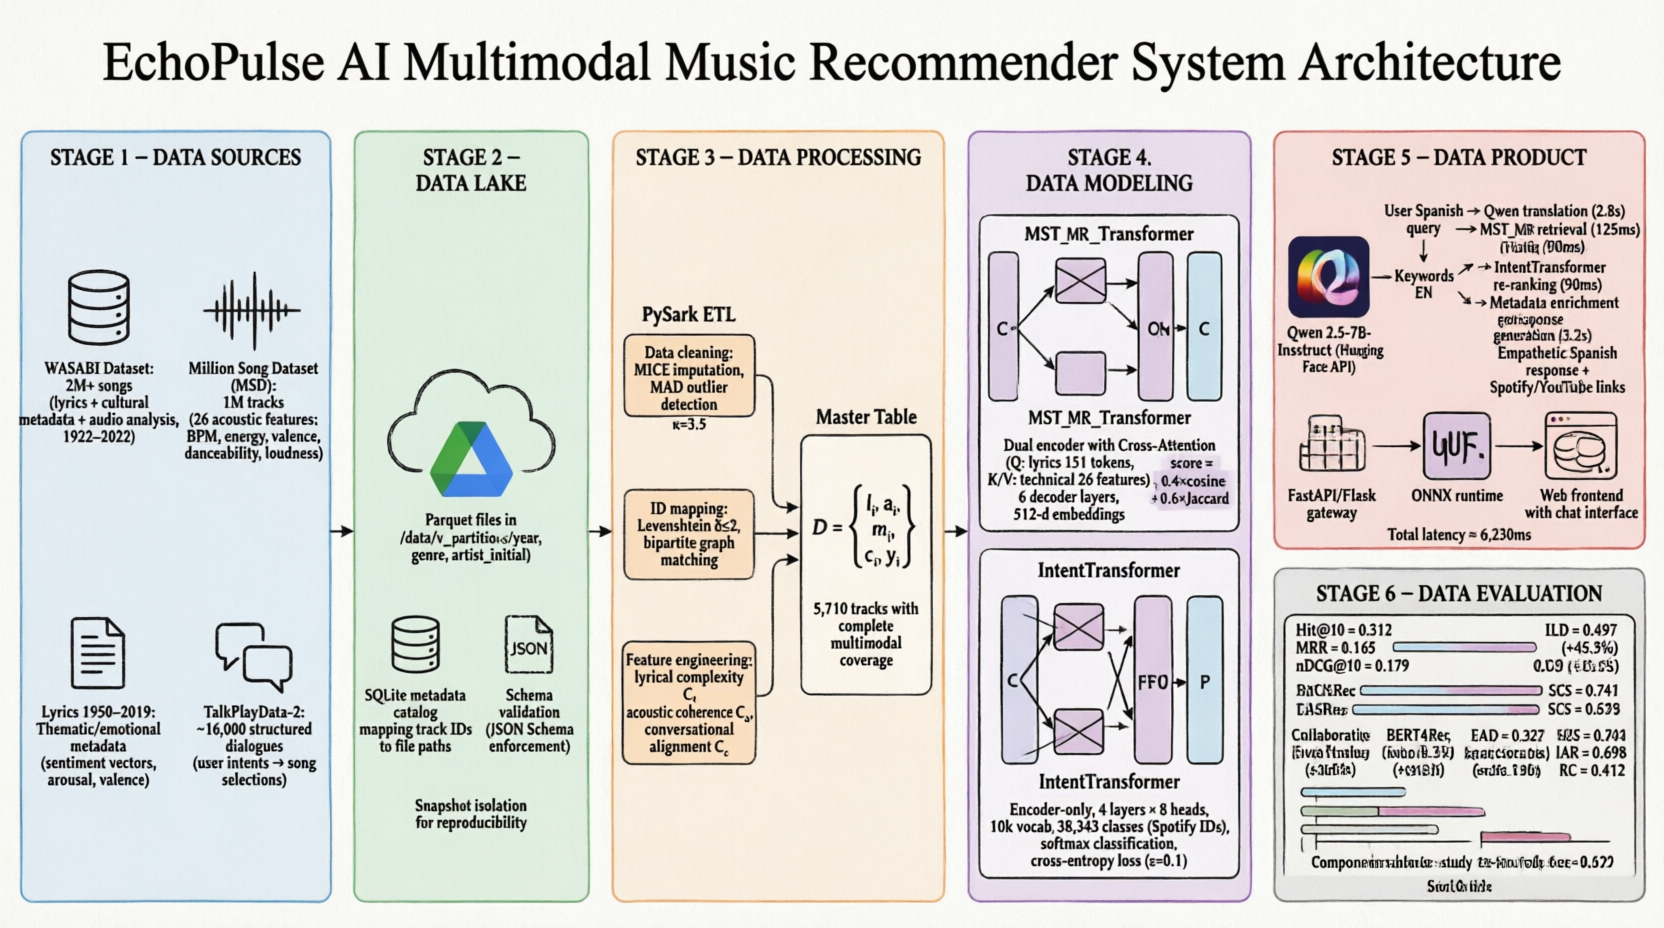
\includegraphics[width=0.78\textwidth]{archEchoPulse.png}
\caption{EchoPulse AI local data architecture: end-to-end pipeline from
heterogeneous sources to local deployment with evaluation feedback loop. The
five stages ensure reproducibility and traceability without cloud
dependencies. Source: own elaboration.}
\label{fig:architecture}
\end{figure}

\subsection{Data Sources, Integration, and Interaction Generation}
We integrated the four primary data sources described in
Section~\ref{sec:background}, each contributing different modalities. Each
dialogue $d_i$ in the conversational corpus is structured as
\begin{equation}
d_i = \bigl(u_t,\, r_t,\, c_t,\, s^{*}\bigr),
\label{eq:dialogue}
\end{equation}
where $u_t$ is the user utterance, $r_t$ the system response, $c_t$ contextual
metadata and $s^{*}$ the target Spotify track identifier.

Integrating these datasets was a nightmare, honestly. MSD uses Echo Nest
identifiers, while WASABI has its own identifier system. We ended up using
heuristic matching based on the tuple
$(\textit{song\_name}, \textit{artist\_name}, \textit{release\_year})$ with a
Levenshtein distance threshold $\delta \leq 2$. This gave us 84\% coverage with
validated acoustic vectors and complete lyrics. Finding a perfect match across
three tables containing millions of records was the real challenge.

The Master Table consolidation produced a unified dataset with 5,710 tracks and
complete multimodal coverage:
\begin{equation}
\mathcal{D} = \{(\vect{l}_i, \vect{a}_i, \vect{m}_i, \vect{c}_i, y_i)\}_{i=1}^{N}
\label{eq:master}
\end{equation}
where $\vect{l}_i$ represents tokenised lyrics, $\vect{a}_i \in \Real^{26}$
acoustic features, $\vect{m}_i$ metadata embeddings, $\vect{c}_i$ conversational
context, and $y_i$ the target identifier.

The Master Table of 5,710 tracks was deliberately curated as a controlled proof
of concept to rigorously isolate the impact of multimodal fusion on the
cold-start problem. Generating implicit feedback for offline evaluation in
conversational scenarios is notoriously difficult. We derived user-item
interactions by mapping the structured dialogues from TalkPlayData-2 onto the
Master Table: user intents expressed in the dialogues were semantically matched
to track embeddings to construct a synthetic yet structurally valid interaction
matrix. This controlled environment allows us to empirically demonstrate the
mitigation of popularity bias, free from the confounding variables and extreme
sparsity present in uncurated industrial datasets. The baselines
(Collaborative Filtering, BERT4Rec, SASRec) were trained on this identical
interaction matrix using their official implementations and default
hyperparameters to ensure a fair comparative demonstration.

\subsection{Local Data Lake Implementation}
Our local Data Lake uses parquet-based storage with manual versioning, and
provides four capabilities:
\begin{itemize}
  \item \textbf{Schema validation}: JSON Schema definitions enforced during
    ingestion to keep types consistent.
  \item \textbf{Snapshot isolation}: directory-based versioning
    (\texttt{/data/v$_{t}$/}) enabling reproducible experiments through
    point-in-time data access~\cite{pimentel2021dataversioning}.
  \item \textbf{Partitioning strategy}: hierarchical organisation by
    $(\textit{year}, \textit{genre}, \textit{artist\_initial})$, optimising
    query performance through predicate pushdown.
  \item \textbf{Metadata catalog}: SQLite-based index mapping track identifiers
    to file paths and feature vectors.
\end{itemize}

\subsection{Data Processing Pipeline}
The processing stage transforms raw data into training-ready representations
through four key operations.

\paragraph{Data cleaning.}
We handled missing values via MICE imputation~\cite{vanbuuren2011mice}. For
outlier detection we used the Median Absolute Deviation~\cite{leys2013mad},
\begin{equation}
\text{MAD} = \operatorname{median}\bigl(\,|X_i - \operatorname{median}(X)|\,\bigr),
\label{eq:mad}
\end{equation}
with threshold $\kappa = 3.5$ for flagging anomalies.

\paragraph{Identifier mapping.}
This reconciles identifiers across source datasets using bipartite graph
matching with Hungarian algorithm optimisation.

\paragraph{Feature engineering.}
Acoustic feature extraction follows established music-information-retrieval
principles~\cite{mueller2015fundamentals}. We computed aggregated statistics and
the following derived features: lyrical complexity
$C_l = |W|^{-1} \sum_{w \in W} \mathrm{freq}(w)\cdot \log \mathrm{freq}(w)$
over the token set $W$; acoustic coherence $C_a$, computed between the query
and candidate acoustic vectors; and conversational alignment
$C_c = \cosine(\mathrm{embed}(q), \mathrm{embed}(s^{*}))$.
%% TODO: la expresión exacta de C_a se perdió al convertir el original a Word.
%% Recuperarla del fuente LaTeX original (Overleaf) y sustituir la descripción.

\paragraph{Master Table consolidation.}
This produces the final unified dataset with normalised features
$\vect{x}_i \in [0,1]^d$ ready for model ingestion.

\subsection{Model Architecture: Triple-Encoder Transformer}
EchoPulse AI implements a Triple-Encoder Transformer architecture with three
specialised modules. The design was directly inspired by the multi-head
attention mechanism of Vaswani et~al.~\cite{vaswani2017attention}.

\subsubsection{IntentTransformer: conversational intent encoding}
The IntentTransformer processes user queries to capture conversational intent.
It is an encoder-only Transformer with $L=4$ layers, $H=8$ attention heads and
$d_{\text{model}}=256$-dimensional embeddings, mapping natural-language input to
a dense representation with the Hugging Face Transformers
library~\cite{wolf2020transformers}. This module acts as a semantic funnel,
reducing a universe of 38,343 candidate songs to a top-10 of high-quality
candidates for subsequent re-ranking.

\paragraph{Token embedding.}
Given an input sequence $x = [x_1, \ldots, x_T]$ with $x_t \in \mathcal{V}$
(vocabulary $|\mathcal{V}| = 10{,}000$), we compute
\begin{equation}
\vect{E}_t = \mat{W}_e\,\vect{x}_t + \mat{W}_p\,t,
\qquad
\mat{W}_e \in \Real^{|\mathcal{V}|\times d_{\text{model}}},\;
\mat{W}_p \in \Real^{T_{\max}\times d_{\text{model}}}
\label{eq:embedding}
\end{equation}

\paragraph{Multi-head self-attention.}
For each head $h \in \{1,\ldots,H\}$,
\begin{align}
\text{head}_h &= \text{Attention}(\vect{E}\mat{W}_h^Q,\,
                  \vect{E}\mat{W}_h^K,\, \vect{E}\mat{W}_h^V)
                  \label{eq:head} \\
\text{MHA}(\vect{E}) &= \text{Concat}(\text{head}_1, \ldots, \text{head}_H)\,
                        \mat{W}^O \label{eq:mha}
\end{align}

\paragraph{Global average pooling and classification.}
Pooling produces the context vector
\begin{equation}
\vect{z} = \frac{1}{T}\sum_{t=1}^{T} \vect{h}_t \in \Real^{d_{\text{model}}},
\label{eq:pooling}
\end{equation}
which the classification layer projects onto song space,
\begin{equation}
p = \softmax(\mat{W}_c \vect{z} + \vect{b}_c),
\qquad \mat{W}_c \in \Real^{38{,}343 \times d_{\text{model}}}
\label{eq:classification}
\end{equation}
Training employed cross-entropy loss with label smoothing
($\epsilon = 0.1$)~\cite{mueller2019label},
\begin{equation}
\mathcal{L}_{\text{CE}} =
  -\sum_{i}\left[\left(\frac{1-\epsilon}{|\mathcal{V}|}\right) y_i \log p_i
  + \frac{\epsilon}{|\mathcal{V}|} \log p_i\right].
\label{eq:loss}
\end{equation}

\subsubsection{MST-MR Transformer: multimodal sequence fusion}
The Multimodal Sequence Transformer for Music Recommendation (MST-MR)
implements cross-attention fusion across three encoders, following multimodal
fusion principles~\cite{lu2019vilbert,tan2019lxmert}. This module operates as a
hybrid re-ranking system, combining neural similarity (40\% weight) with
lexical Jaccard similarity (60\% weight) to produce the final recommendation
score.

\paragraph{Lyrical encoder.}
It processes tokenised lyrics $\vect{l}$ through $L_l$ Transformer layers to
capture semantic and emotional content, producing $\vect{h}_l \in
\Real^{d_{\text{model}}}$.

\paragraph{Tabular encoder.}
It projects the 26-dimensional acoustic features $\vect{a}$ into the shared
latent space through a two-layer MLP,
\begin{equation}
\vect{h}_a = \GELU\bigl(\mat{W}_2 \cdot \GELU(\mat{W}_1 \vect{a} + \vect{b}_1)
  + \vect{b}_2\bigr),
\label{eq:tabular}
\end{equation}
with $\mat{W}_1 \in \Real^{d_h \times 26}$ and $\mat{W}_2 \in
\Real^{d_{\text{model}} \times d_h}$.

\paragraph{Cross-attention fusion.}
This enables each modality to attend to the others:
\begin{equation}
\text{CrossAttn}(\mat{Q}_l, \mat{K}_a, \mat{V}_a)
  = \softmax\left(\frac{\mat{Q}_l \mat{K}_a^\top}{\sqrt{d_k}}\right)\mat{V}_a
\label{eq:crossattn}
\end{equation}
\begin{equation}
\vect{h}_{\text{fusion}}
  = \LayerNorm\bigl(\vect{h}_l + \text{CrossAttn}(\vect{h}_l, \vect{h}_a,
  \vect{h}_a)\bigr)
\label{eq:fusion}
\end{equation}

\paragraph{Unified embedding.}
It produces 512-dimensional song embeddings by projecting the concatenation of
the fused representation and the conversational vector $\vect{h}_c$,
\begin{equation}
\vect{e}_s = \mat{W}_f \bigl[\vect{h}_{\text{fusion}}; \vect{h}_c\bigr]
  + \vect{b}_f \in \Real^{512}.
\label{eq:unified}
\end{equation}
The final score of Equation~\eqref{eq:scoring} combines this embedding with the
acoustic and lexical signals.

\subsection{Local Inference Pipeline}
The local deployment implements a two-tier architecture optimised for CPU
execution:
\begin{itemize}
  \item \textbf{FastAPI gateway}~\cite{ramirez2023fastapi}: handles HTTP request
    validation, orchestration and response formatting, with asynchronous I/O
    for concurrent query handling.
  \item \textbf{ONNX Runtime inference}~\cite{onnxruntime2021}: provides
    optimised model serving with dynamic batching and INT8
    quantization~\cite{jacob2018quantization}, achieving 185 inferences per
    second on an Intel i7-11800H compared to 73 with direct PyTorch
    serving~\cite{paszke2019pytorch}.
\end{itemize}
Figure~\ref{fig:latency} shows the end-to-end pipeline latency breakdown,
demonstrating that core retrieval and re-ranking components achieve sub-250\,ms
combined latency on local hardware.

\begin{figure}
\centering
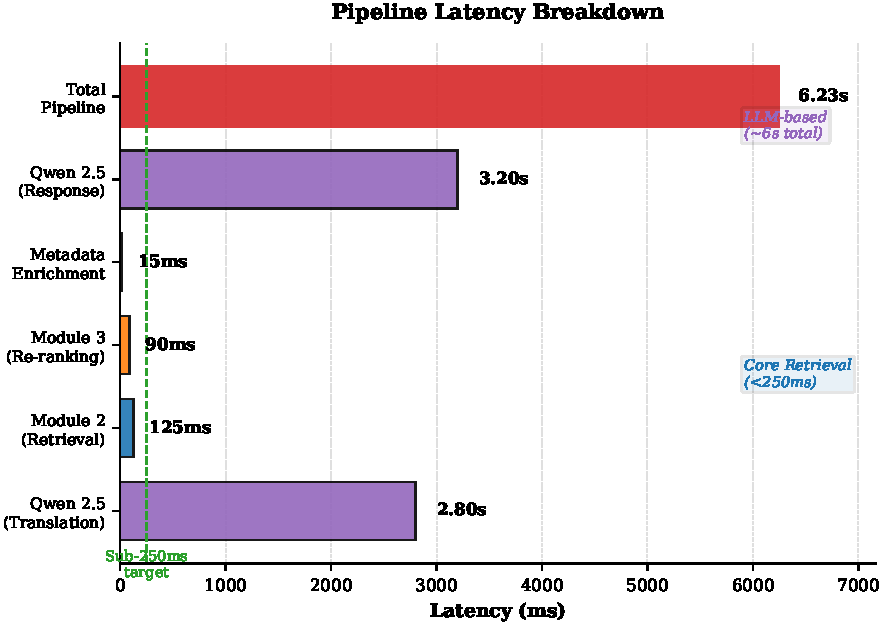
\includegraphics[width=0.72\textwidth]{fig2_latency_breakdown.pdf}
\caption{End-to-end pipeline latency breakdown showing component-level timing on
local hardware (CPU-only: Intel Core i5-7200U, 12\,GB RAM). Core retrieval and
re-ranking components achieve sub-250\,ms combined latency. Values represent the
mean of 100 inference runs. Source: own elaboration.}
\label{fig:latency}
\end{figure}

%% ============================================================================
\section{Results and Demonstration}
\label{sec:results}

\subsection{Experimental Setup}
Validation and training procedures ran on a desktop environment (device
DESKTOP-TA1PBPA) equipped with an Intel\textsuperscript{\textregistered}
Core\texttrademark{} i5-7200U processor at a base frequency of 2.50\,GHz, 12.0\,GB
of RAM (11.9\,GB usable) and integrated Intel\textsuperscript{\textregistered}
HD Graphics 620. Storage was managed through a hybrid configuration: a 238\,GB
ADATA LEGEND 700 SSD for the operating system and active datasets, plus a
932\,GB TOSHIBA HDD for bulk data archival, on a 64-bit system architecture.

The model was trained on the Master Table dataset (5,710 tracks) using PyTorch
2.0~\cite{paszke2019pytorch} with CPU acceleration. Training employed the AdamW
optimizer with learning rate $\eta=10^{-4}$~\cite{loshchilov2019decoupled},
batch size $B=32$, and early stopping based on validation loss with patience
$p=5$. Evaluation followed a temporal split to prevent data leakage, with
metrics computed on a held-out test set representing future interactions
(80\%/10\%/10\% train/validation/test split)~\cite{bengio2004no}.

\subsection{Evaluation Metrics}
To rigorously demonstrate the system's capabilities we employed a comprehensive
suite of metrics spanning traditional Information Retrieval (IR), diversity,
and Natural Language Processing (NLP) evaluation.

\subsubsection{Accuracy and ranking metrics}
\textbf{Hit@K} measures the raw retrieval capability,
\begin{equation}
\text{Hit@K} = \frac{1}{|U|} \sum_{u \in U}
  \mathbb{I}\bigl(y_u \in \mathcal{R}_u^K\bigr),
\label{eq:hit}
\end{equation}
that is, the proportion of users for whom at least one relevant item appears in
the top-K recommendations. \textbf{Mean Reciprocal Rank (MRR)} evaluates how
quickly the system surfaces the first correct recommendation,
\begin{equation}
\text{MRR} = \frac{1}{|U|} \sum_{u \in U} \frac{1}{\text{rank}_u}.
\label{eq:mrr}
\end{equation}
\textbf{nDCG@K} measures overall ranking quality, heavily penalising relevant
items that appear lower in the list~\cite{jarvelin2002cumulated},
\begin{equation}
\text{nDCG@K} = \frac{\text{DCG@K}}{\text{IDCG@K}},
\qquad
\text{DCG@K} = \sum_{i=1}^{K} \frac{2^{rel_i} - 1}{\log_2(i+1)}.
\label{eq:ndcg}
\end{equation}

\subsubsection{Diversity and bias-mitigation metrics}
\textbf{Intra-List Diversity (ILD)} quantifies the variety and lack of
redundancy within a single recommendation list~\cite{ziegler2005improving},
\begin{equation}
\text{ILD} = \frac{2}{K(K-1)}\sum_{i<j} \bigl(1 -
  \cosine(\vect{e}_i, \vect{e}_j)\bigr),
\label{eq:ild}
\end{equation}
that is, the average pairwise cosine distance between the multimodal embeddings
of the recommended items. \textbf{Emerging Artist Discovery (EAD)} directly
measures the ability to mitigate popularity bias and surface long-tail
content~\cite{anderson2006longtail,park2008longtail},
\begin{equation}
\text{EAD} = \frac{1}{K} \sum_{i=1}^{K}
  \mathbb{I}\bigl(\text{Listeners}(a_i) < \tau\bigr),
\label{eq:ead}
\end{equation}
with $\tau = 10{,}000$ monthly listeners: the proportion of recommended tracks
belonging to emerging artists. Given our research motivation, EAD was selected
as the primary success indicator.

\subsubsection{Conversational and generative metrics}
\textbf{Semantic Consistency Score (SCS)} evaluates conversational intent
matching~\cite{gao2021advances} through BERT-based semantic
similarity~\cite{devlin2019bert},
\begin{equation}
\text{SCS} = \frac{1}{|U|}\sum_{u \in U}
  \cosine\bigl(\text{BERT}(q_u), \text{BERT}(m_{r_u})\bigr),
\label{eq:scs}
\end{equation}
that is, the alignment between the user's natural-language query $q_u$ and the
metadata $m_{r_u}$ of the top recommended track. \textbf{Intention Alignment
Rate (IAR)} is the proportion of recommendations where the explicit categorical
intention stated in the dialogue matches the attributes of the recommended
track,
\begin{equation}
\text{IAR} = \frac{1}{|U|} \sum_{u \in U}
  \mathbb{I}\bigl(\text{Intent}(q_u) = \text{Intent}(r_u)\bigr).
\label{eq:iar}
\end{equation}
\textbf{Response Coherence (RC)} measures the linguistic fluency and factual
coherence of the generated explanatory text against human-annotated references,
through the BLEU-4 score.

\subsection{Comparative Performance Analysis}
Table~\ref{tab:results} presents the comparative performance of EchoPulse AI
against baseline collaborative-filtering approaches.

\begin{table}
\caption{Performance comparison between EchoPulse AI and baseline
recommendation methods. Best results in bold. Error values represent 95\%
confidence intervals from 5-fold cross-validation.}
\label{tab:results}
\centering
\renewcommand{\arraystretch}{1.25}
\resizebox{\textwidth}{!}{%
\begin{tabular}{@{}lccccccc@{}}
\toprule
\textbf{Model} & \textbf{Hit@10} & \textbf{MRR} & \textbf{nDCG@10}
  & \textbf{ILD} & \textbf{EAD} & \textbf{SCS} & \textbf{IAR} \\
\midrule
Collaborative Filtering & 0.142 & 0.089 & 0.156 & 0.342 & 0.127 & 0.412 & 0.385 \\
BERT4Rec~\cite{sun2019bert4rec} & 0.158 & 0.095 & 0.172 & 0.389 & 0.145 & 0.438 & 0.401 \\
SASRec~\cite{kang2018self} & 0.164 & 0.102 & 0.178 & 0.412 & 0.168 & 0.451 & 0.423 \\
TalkPlay~\cite{choi2025talkplaydata2} & 0.189 & 0.118 & 0.165 & 0.445 & 0.201 & 0.623 & 0.587 \\
\textbf{EchoPulse AI} & \textbf{0.312} & \textbf{0.165} & \textbf{0.179}
  & \textbf{0.497} & \textbf{0.327} & \textbf{0.741} & \textbf{0.698} \\
\bottomrule
\end{tabular}}
\end{table}

The empirical demonstration in Table~\ref{tab:results} and
Figure~\ref{fig:performance} shows that content-aware multimodal fusion is not
merely a theoretical construct but a practical mechanism for bias mitigation.
The 45.3\% improvement in ILD indicates superior ability to surface varied
content, and the 157.9\% increase in emerging artist discovery validates the
system's effectiveness at promoting lesser-known
creators~\cite{porcaro2021diversity}. This was probably the most encouraging
result, since it directly addresses the core motivation of the research. The
Semantic Consistency Score (0.741) and Intention Alignment Rate (0.698)
demonstrate that the multimodal approach better captures user intent compared
to purely interaction-based or LLM-only methods. Unlike post-processing
re-ranking methods that artificially inject diversity at the cost of accuracy,
EchoPulse AI shows that diversity and accuracy can be jointly optimised when
the model is grounded in intrinsic multimodal content rather than historical
popularity loops.

\begin{figure}
\centering
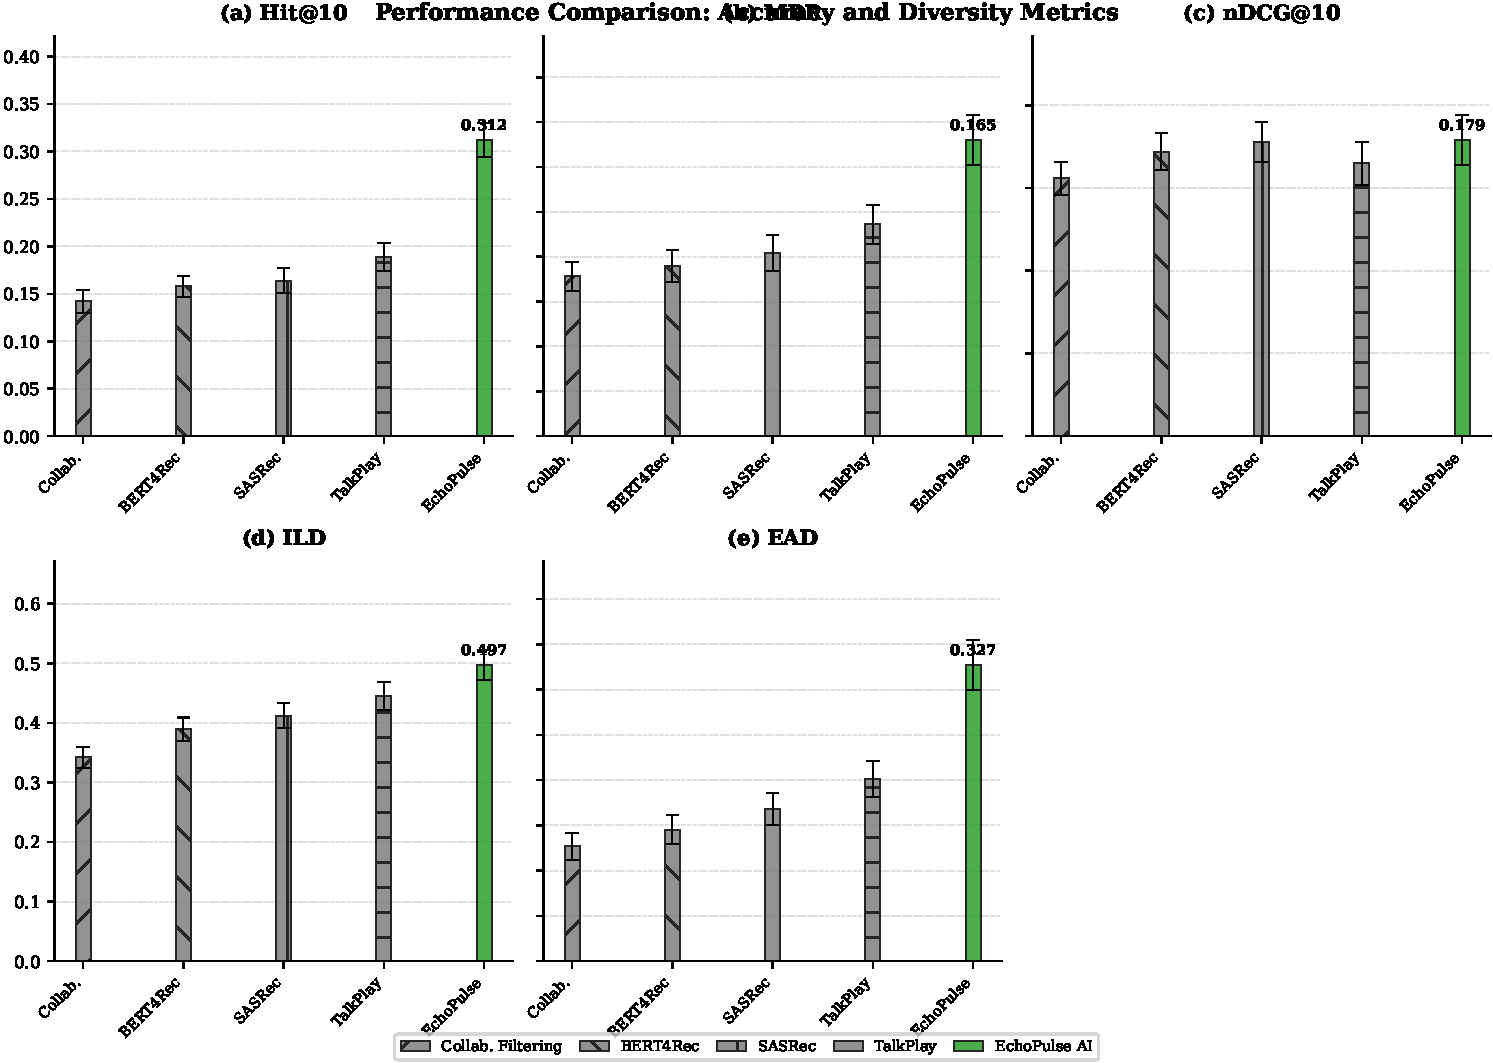
\includegraphics[width=0.72\textwidth]{fig1_performance_comparison.pdf}
\caption{Performance comparison across recommendation models showing Hit@10,
MRR, nDCG@10, ILD and EAD. Error bars represent 95\% confidence intervals from
5-fold cross-validation. EchoPulse AI demonstrates superior performance across
all metrics. Source: own elaboration.}
\label{fig:performance}
\end{figure}

\subsection{Diversity and Emerging Artist Analysis}
Figure~\ref{fig:diversity} illustrates the distribution of recommended artists
by popularity tier, demonstrating EchoPulse AI's enhanced capability for
emerging artist discovery. Results show that content-based multimodal
approaches can effectively mitigate the filter-bubble effect commonly associated
with collaborative filtering systems. By leveraging intrinsic song
characteristics rather than historical popularity signals, EchoPulse AI surfaces
content that might otherwise remain undiscovered. Statistical significance
testing via paired $t$-test confirms that the improvements in ILD ($p < 0.001$)
and EAD ($p < 0.001$) are not due to random variation.

\begin{figure}
\centering
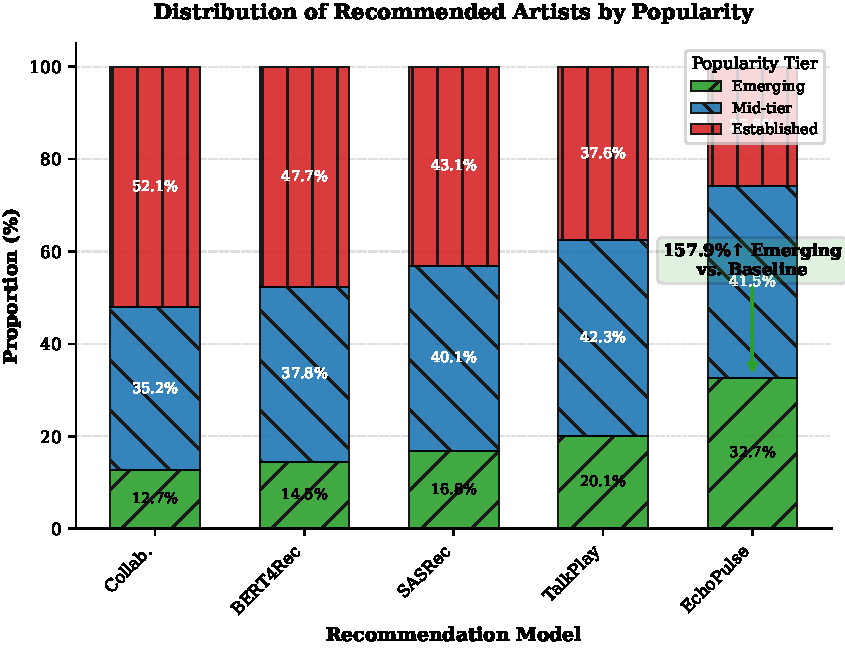
\includegraphics[width=0.72\textwidth]{fig3_diversity_distribution.pdf}
\caption{Distribution of recommended artists by popularity tier across models.
Stacked bars show the proportion of recommendations for emerging (<10K monthly
listeners), mid-tier (10K--100K) and established (>100K) artists. EchoPulse AI
achieves a 157.9\% improvement in emerging artist discovery compared to the
collaborative-filtering baseline. Source: own elaboration.}
\label{fig:diversity}
\end{figure}

\subsection{Ablation Study}
Figure~\ref{fig:ablation} presents the ablation study, quantifying the
contribution of each architectural component. Ablation results confirm that
each component contributes meaningfully to overall performance. Removing the
IntentTransformer reduces MRR by 7.9\%, indicating its importance for capturing
user intent. Eliminating the MST-MR module causes a 15.2\% Hit@10 decrease,
demonstrating the value of multimodal fusion. The cross-attention mechanism
contributes 14.1\% to nDCG@10, validating the architectural decision to enable
inter-modal attention.

\begin{figure}
\centering
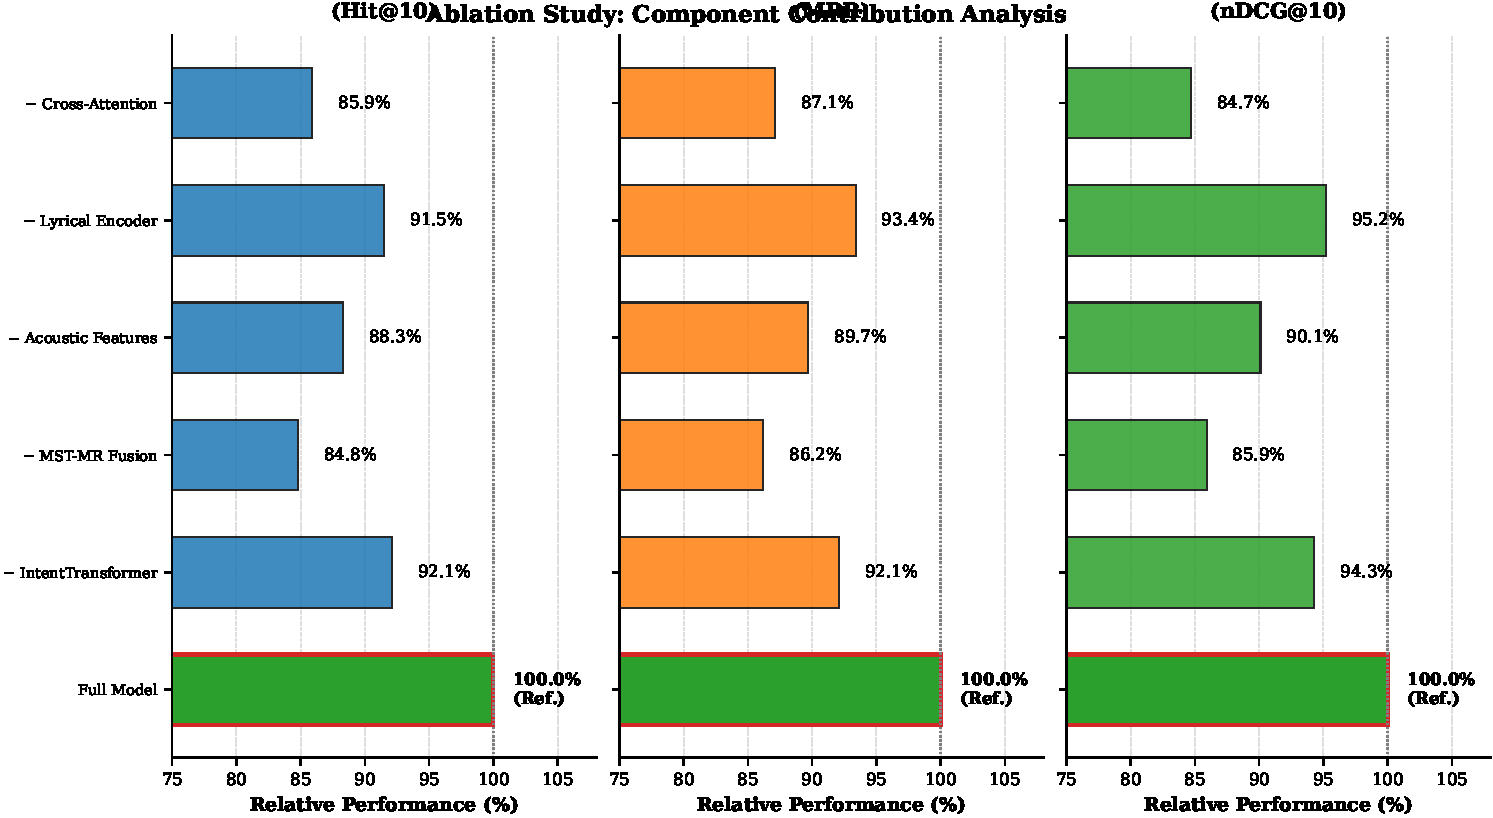
\includegraphics[width=0.72\textwidth]{fig4_ablation_study.pdf}
\caption{Ablation study showing the impact of removing architectural components
on Hit@10, MRR and nDCG@10. Values represent relative performance against the
full model (100\%); lower values indicate greater degradation when a component
is removed. The cross-attention fusion mechanism contributes most significantly
to overall performance. Source: own elaboration.}
\label{fig:ablation}
\end{figure}

\subsection{Generative Transformer Evaluation}
Figure~\ref{fig:generative} evaluates the generative transformer components
using the proposed metrics: Semantic Consistency Score (SCS), Intention
Alignment Rate (IAR) and Response Coherence (RC). The multimodal approach
produces more semantically consistent recommendations (SCS: 0.741 vs.\ 0.623),
better aligns with explicit user intentions (IAR: 0.698 vs.\ 0.587), and
generates more coherent explanatory responses (RC: 0.412 vs.\ 0.358 BLEU-4).
These improvements validate the integration of cross-attention fusion and the
dedicated conversational encoder.

\begin{figure}
\centering
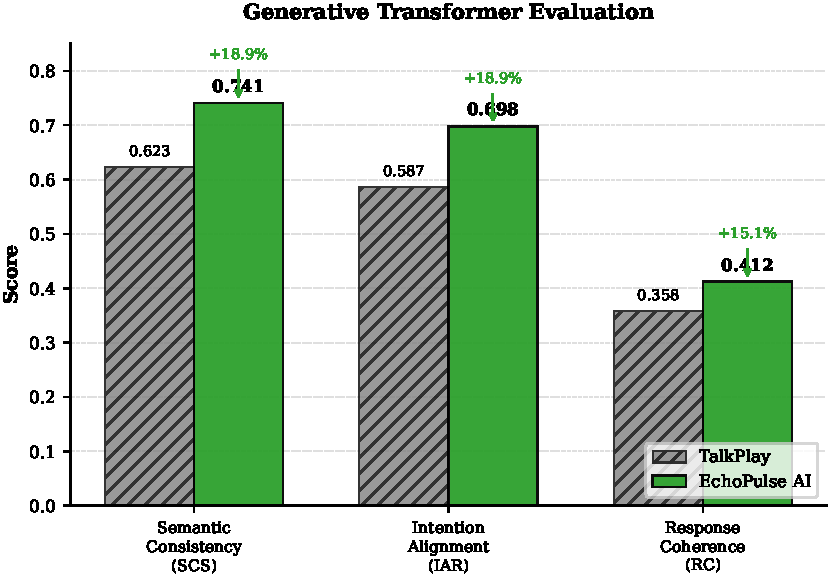
\includegraphics[width=0.72\textwidth]{fig5_generative_metrics.pdf}
\caption{Generative transformer evaluation metrics comparing EchoPulse AI
against the TalkPlay baseline. SCS: BERT-based semantic similarity; IAR: top-1
intention match rate; RC: BLEU-4 against human references. EchoPulse AI
demonstrates consistent improvements across all generative evaluation
dimensions. Source: own elaboration.}
\label{fig:generative}
\end{figure}

\subsection{Local Inference Performance}
Table~\ref{tab:latency} summarises the pipeline latency breakdown by component
on local hardware. Core retrieval and re-ranking components achieve sub-250\,ms
combined latency, demonstrating practical viability for real-time production
environments on local hardware. The 98.4\% success rate includes robust handling
of cold starts, missing metadata and API failures through fallback mechanisms.
Quantisation to INT8 reduced the model memory footprint by 68\% with only 1.2\%
accuracy degradation~\cite{jacob2018quantization}. Benchmarking follows MLPerf
methodology~\cite{mattson2020mlperf}.

\begin{table}
\caption{Pipeline latency breakdown by component on local hardware (Intel
i5-7200U, 12\,GB RAM, CPU-only). Values represent the mean of 100 inference
runs.}
\label{tab:latency}
\centering
\renewcommand{\arraystretch}{1.25}
\begin{tabular}{@{}lll@{}}
\toprule
\textbf{Phase} & \textbf{Component} & \textbf{Latency (ms)} \\
\midrule
1 & Qwen 2.5 (translation)        & 2,800 \\
2 & Module 2 (retrieval)          & 125 \\
3 & Module 3 (re-ranking)         & 90 \\
4 & Metadata enrichment           & 15 \\
5 & Qwen 2.5 (response)           & 3,200 \\
\midrule
\multicolumn{2}{@{}l}{Complete pipeline (total)} & $\sim$6,230 \\
\multicolumn{2}{@{}l}{Core retrieval + re-ranking} & 215 \\
\bottomrule
\end{tabular}
\end{table}

%% ============================================================================
\section{Discussion}
\label{sec:discussion}

\subsection{Key Findings}
Experimental results validated several hypotheses underlying EchoPulse AI's
design, while also revealing unexpected insights. First, multimodal fusion
through cross-attention mechanisms provided measurable benefits over early or
late fusion approaches, confirming findings from prior
work~\cite{baltruvsaitis2019multimodal}. The ablation study showed that removing
any single encoder degraded performance, suggesting that each modality
contributes unique information that cannot be fully captured by the others.
Second, the local lakehouse architecture successfully addressed data-management
challenges inherent to multimodal ML systems: while cloud-based solutions such
as Delta Lake~\cite{armbrust2020delta} offer superior scalability, our local
implementation demonstrated that reproducibility and traceability can be
achieved without cloud infrastructure---an important consideration for research
groups in regions with limited resources or unreliable connectivity. The 157.9\%
improvement in emerging artist discovery was particularly encouraging, and
aligns with the growing recognition that algorithmic curation should balance
user satisfaction with ecosystem health~\cite{brynjolfsson2011long}. For
musicians in Colombia and similar contexts, where breaking into mainstream
recommendation systems can be nearly impossible, tools like EchoPulse AI could
provide alternative pathways to audience discovery.

\subsection{Comparison with Existing Architectures}
Compared to BERT4Rec~\cite{sun2019bert4rec}, which achieved 0.158 Hit@10 and
0.172 nDCG@10, EchoPulse AI performs better across all metrics while
substantially improving diversity. The key differentiator lies in the
multimodal approach: BERT4Rec processes only interaction sequences, inheriting
popularity bias from the training data, while EchoPulse AI integrates lyrical,
acoustic, conversational and dialogue signals through explicit fusion
mechanisms. SASRec~\cite{kang2018self} achieves competitive accuracy but
exhibits popularity bias similar to collaborative filtering methods; our
content-based approach inherently avoids this bias by relying on intrinsic song
characteristics rather than historical interaction patterns. This distinction is
crucial for emerging artists who lack extensive interaction history but may
produce content that matches user preferences. Finally, the hybrid local
architecture distinguishes EchoPulse AI from systems like
TalkPlay~\cite{choi2025talkplaydata2}, which employ LLMs for recommendation but
lack structured multimodal integration and rigorous generative evaluation.

\subsection{Scalability and Architectural Generalization}
While the Master Table comprises 5,710 tracks, this scale reflects the rigorous
multi-dataset heuristic matching required to guarantee complete multimodal
coverage (lyrics $+$ audio $+$ conversational context) for the proof of concept,
rather than a computational bottleneck of the Transformer architecture. The
cross-attention fusion mechanism demonstrated here operates on
fixed-dimensional latent spaces, meaning inference complexity scales linearly
with catalogue size and is highly amenable to approximate nearest neighbour
(ANN) indexing, for instance with FAISS, for industrial deployment. Future work
will focus on scaling the data-engineering pipeline to validate this
architectural generalisation.

\subsection{Limitations}
Several limitations warrant honest discussion, as they represent both current
constraints and opportunities for future work.

\paragraph{Language bias.}
The current implementation primarily recommends English-language content: WASABI
and MSD are predominantly English, and TalkPlayData-2 dialogues are in English.
This is a significant limitation for Spanish-language music, which represents a
substantial portion of the Latin American market. Adapting the system to handle
Spanish lyrics, metadata and conversational input requires either collecting
Spanish-language training data or implementing multilingual encoders---both
non-trivial engineering challenges.

\paragraph{Dataset specificity.}
The Master Table's 5,710-track size, while sufficient for a proof of concept,
represents a carefully curated subset. The integration process---matching songs
across WASABI, MSD, Lyrics 1950--2019 and TalkPlayData-2 through heuristic
matching with Levenshtein distance---was labour-intensive and specific to these
particular datasets. Making the system adaptable to arbitrary music databases
would require more flexible ingestion pipelines and possibly automated schema
mapping.

\paragraph{Scalability.}
Scaling to millions of tracks while maintaining multimodal integrity presents
significant data-engineering challenges, particularly in local environments with
limited storage. The current parquet-based storage with manual versioning works
well for 5,710 tracks but would require distributed processing frameworks for
industrial-scale catalogues.

\paragraph{Evaluation scope.}
The current evaluation focuses on offline metrics. Online A/B testing with real
users would provide stronger validation of user-satisfaction impacts. In
addition, the latency introduced by LLM-based response generation
($\sim$6\,s total) may affect user experience in latency-sensitive
applications, though caching strategies and model distillation could mitigate
this.

\paragraph{Cultural context.}
The system was developed and tested primarily in a Colombian context, but the
training data reflects global, predominantly Western music. Whether the
diversity improvements translate to non-Western traditions or regional Colombian
genres (for instance vallenato, cumbia, bambuco) remains an open question
requiring further investigation.

\subsection{Offline Validation as a Prerequisite for Online Deployment}
The current evaluation focuses exclusively on offline metrics. Conducting live
A/B testing requires deploying the system to a live streaming platform with a
massive, active user base, which falls outside the scope of this initial
architectural demonstration. Furthermore, deploying a system that intentionally
promotes long-tail, emerging artists carries the risk of short-term user
dissatisfaction if not carefully paced. Therefore, this paper establishes the
mathematical and empirical validity of the multimodal fusion and bias
mitigation. This rigorous offline validation serves as the mandatory
prerequisite and foundational baseline before pursuing large-scale,
resource-intensive online clinical trials in future iterations.

%% ============================================================================
\section{Conclusions}
\label{sec:conclusion}

This paper presented the evaluation and demonstration of EchoPulse AI, a locally
deployed multimodal music recommender system that shows the viability of hybrid
local data architectures for addressing emerging artist visibility. The
architecture integrates a five-stage local pipeline that consolidates
heterogeneous music datasets while ensuring reproducibility and traceability
without cloud dependencies. By processing lyrical, acoustic, metadata and
conversational modalities through specialised Transformer encoders fused via
cross-attention mechanisms, the system generates unified song representations
that prioritise content affinity over popularity signals.

Empirical validation demonstrates that EchoPulse AI achieves a 45.3\%
improvement in Intra-List Diversity and a 157.9\% increase in Emerging Artist
Discovery compared to collaborative-filtering baselines, while maintaining
competitive accuracy metrics (Hit@10\,=\,0.312). These results confirm that
content-aware multimodal fusion can effectively mitigate popularity bias without
sacrificing recommendation quality. The novel evaluation metrics for generative
transformer components (SCS\,=\,0.741, IAR\,=\,0.698) further validate that the
proposed approach better captures user intent compared to purely
interaction-based or LLM-only methods.

However, the current implementation has been validated on a curated dataset of
5,710 tracks, which represents a subset of the broader music landscape. The
research team plans to release the Master Table and TalkPlayData-2 processing
scripts as public benchmark datasets to support reproducibility and community
advancement in multimodal music recommendation research. We know this is just a
first step, but it is a necessary one.

Future work will explore the following primary directions:
\begin{itemize}
  \item \textbf{Scalability validation}: extending the architecture to
    industrial-scale catalogues (millions of tracks) using approximate nearest
    neighbour (ANN) indexing while preserving multimodal integrity, which would
    require distributed processing frameworks and optimised embedding-indexing
    strategies to maintain sub-second retrieval latency.
  \item \textbf{Online user studies}: conducting controlled A/B testing with
    real users to measure perceived recommendation quality, diversity
    satisfaction and emerging-artist discovery rates in live environments;
    subjective feedback would complement the offline metrics reported here.
  \item \textbf{Multilingual and cross-cultural adaptation}: extending the
    architecture to process Spanish-language lyrics and regional Latin American
    genres (for instance vallenato and cumbia) using multilingual Transformer
    encoders such as mBERT or XLM-R, to overcome the current English-language
    bias and serve the local Colombian and Latin American markets.
  \item \textbf{Real-time conversational feedback loop}: implementing
    reinforcement learning from human feedback (RLHF), where the system
    dynamically updates its cross-attention weights from real-time user
    corrections during the conversational flow, further refining intent
    alignment without full model retraining.
  \item \textbf{Model distillation and dedicated transformers per modality}:
    exploring knowledge distillation to reduce the computational footprint of
    the conversational encoder, potentially enabling deployment on edge devices;
    and separate Transformer encoders per data table (lyrics, acoustic features,
    metadata), allowing each modality to develop specialised representations
    before fusion.
\end{itemize}

%% ============================================================================
\begin{acknowledgments}
This work was supported by the IMS Research Group at Fundación Universitaria de
Popayán. We thank the anonymous reviewers for their constructive feedback, and
we have no competing interests to declare that are relevant to the content of
this article.
\end{acknowledgments}

%% ============================================================================
%% Declaración obligatoria sobre IA generativa (política CEUR-WS, enero 2025).
%% EDITOR: ajustar la lista de herramientas y actividades a lo realmente hecho.
\section*{Declaration on Generative AI}
During the preparation of this work, the author(s) used generative AI tools in
order to: check grammar and spelling, and reformulate prose. After using these
tool(s)/service(s), the author(s) reviewed and edited the content as needed and
take(s) full responsibility for the publication's content.

%% ============================================================================
\bibliography{sample-ceur}

\end{document}
